\begin{figure}
	\centering
	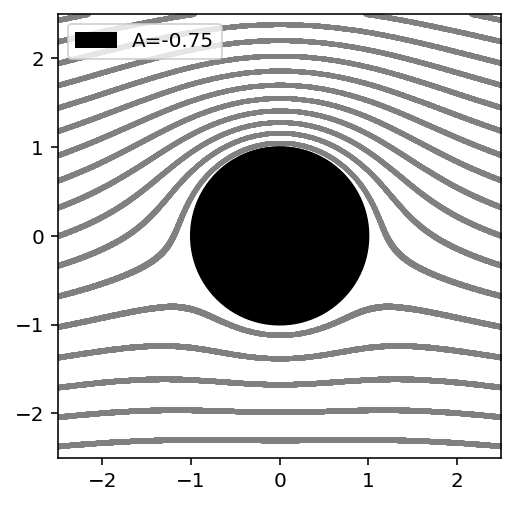
\includegraphics[width=0.45\textwidth]{papers/joukowski/images/05_stroemungslinien/Magnus_Strom_A075_g.png}
	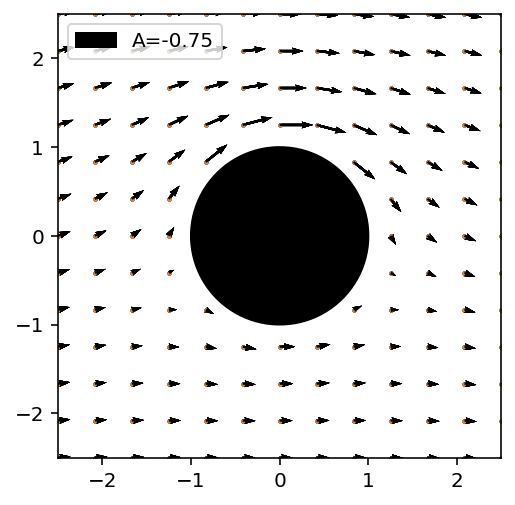
\includegraphics[width=0.45\textwidth]{papers/joukowski/images/05_stroemungslinien/Magnus_Speed_A075.png}
	\caption{
		Durch das Rotieren des Zylinders entsteht eine Asymmetrie in den Strömungslinien.
		Diese Asymmetrie führt dazu,
		dass die Geschwindigkeit ober- und unterhalb des Zylinders nicht mehr gleichmässig zunehmen.
		\label{joukowski:Stroemungslinien:fig_magnus}
	}
\end{figure}
